% 例 2：Rt△ABC, ∠ABC=90°, O=AC 中点, 延长 BO 到 D 使 OD=OB, 构造矩形 ABCD'
% 实际构造的是矩形 ABCD（不是题目原符号；这里用 D 表示新点）
\documentclass[tikz,border=4pt]{standalone}
\usepackage{ctex}
\usepackage{amsmath}
\usetikzlibrary{calc, decorations.markings}
\begin{document}
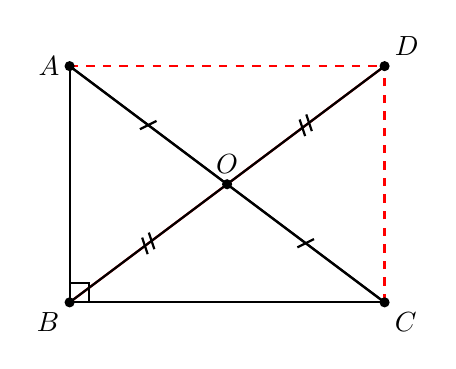
\begin{tikzpicture}[scale=1.0, thick,
  tickone/.style={postaction={decorate, decoration={markings,
    mark=at position 0.5 with {\draw (-1.5pt,-3pt) -- (1.5pt,3pt);}}}},
  ticktwo/.style={postaction={decorate, decoration={markings,
    mark=at position 0.5 with {\draw (-2.5pt,-3pt) -- (-0.5pt,3pt);
                               \draw (0.5pt,-3pt)  -- (2.5pt,3pt);}}}},
]
  % 直角三角形 A(0,3) B(0,0) C(4,0)
  \coordinate (A) at (0,3);
  \coordinate (B) at (0,0);
  \coordinate (C) at (4,0);
  \coordinate (O) at ($(A)!0.5!(C)$);
  % D = 2O - B（即 B 关于 O 的对称点），落在 (4,3)，构成矩形
  \coordinate (D) at (4,3);
  % 原三角形 ABC 实线
  \draw (A) -- (B) -- (C);
  \draw (A) -- (C);
  % 辅助延长线（红色）
  \draw[red, thick] (B) -- (D);
  \draw[red, thick, dashed] (A) -- (D);
  \draw[red, thick, dashed] (C) -- (D);
  % OB = OD 标记
  \draw[ticktwo] (B) -- (O);
  \draw[ticktwo] (O) -- (D);
  % OA = OC 标记
  \draw[tickone] (A) -- (O);
  \draw[tickone] (O) -- (C);
  % 直角标记 B
  \draw (0.25,0) -- (0.25,0.25) -- (0,0.25);
  \foreach \pt in {A,B,C,D,O} \filldraw (\pt) circle (1.4pt);
  \node[left]  at (A) {$A$};
  \node[below left] at (B) {$B$};
  \node[below right] at (C) {$C$};
  \node[above right] at (D) {$D$};
  \node[above] at (O) {$O$};
\end{tikzpicture}
\end{document}
